\documentclass[runningheads]{llncs}

\usepackage{graphicx}
\usepackage{amssymb,amsmath}
\usepackage{array}
\usepackage{booktabs}
\usepackage{adjustbox,lipsum}
\usepackage{multirow}
\usepackage{soul}
\usepackage{algorithm}
\usepackage{algorithmicx}
\usepackage{algpseudocode}
\usepackage{lscape}
\usepackage{listings}
\usepackage{verbatim}
\usepackage{subfigure}
\usepackage{comment}
\usepackage{url}
\usepackage{hyperref}

\usepackage[utf8]{inputenc}
\usepackage[T1]{fontenc} 
\usepackage[spanish]{babel}

\begin{document}

\title{Detección de ``insiders'' utilizando metodologías de aprendizaje máquina}

\titlerunning{InsidersVsMachineLearning}
\author{Ulises Jiménez, José M. Sarmiento}
\authorrunning{U. Jiménez, \and J. Sarmiento}

\institute{Universidad Panamericana, Facultad de Ingenier\'{i}a,\\Augusto Rodin 498, Ciudad de M\'{e}xico, 03920, M\'{e}xico
\email{0231936@up.edu.mx, 0231932@up.edu.mx}}

\maketitle              

\begin{abstract}
Este trabajo presenta cómo el aprendizaje de máquina puede detectar comportamientos de empleados fraudulentos a partir de su huella digital. Para generar el modelo se utilizaron datos sintéticos y se probaron cuatro modelos de aprendizaje de máquina, a saber, regresión logística con gradiente estocástico, máquinas de soporte vectorial, bosques aleatorios y XGBoost. El modelo que mejor detecta a los ``Insiders''` para el conjunto de datos analizado fue el de bosque aleatorio que ha mostrado un buen desempeño para diferentes problemas.

% Máximo 5 palabras clave
\keywords{Fraude \and Fraude Interno \and Aprendizaje Máquina \and Detección de anomalías}
\end{abstract}

%%%%%%%%%%%%%%%%%%%%%%%%%%%%%%%%%%%%%%%%%%%%%%%%%
\section{Introducción}
\label{sec:introduccion}

Los empleados fraudulentos representan una amenaza sustancial para los servicios financieros por su conocimiento y acceso a sistemas internos y datos sensibles. El fraude interno es perpetrado por empleado, ex empleado, un proveedor o algún socio comercial que tiene o ha tenido acceso autorizado a la red, los datos o los sistemas y que intencionalmente ha hecho un mal uso que afecte la confidencialidad, integridad o disponibilidad de los sistemas o información de la empresa. De acuerdo a \cite{insfreqcost} el costo promedio de un incidente que involucra a un empleado o proveedor negligente es de \$283,281 USD, el costo es más del doble \$648,845 si el incidente involucra a un ladrón ("Thief") o impostor y finalmente los incidentes por Hackers le cuestan a las organizaciones en promedio \$607,745.

La detección de la amenaza de fraude interno o 'insider' es un reto extremadamente complejo debido a que, primero los insiders hacen cosas no autorizadas con el uso de sus accesos legítimos; por lo tanto, controles de seguridad como detección de intrusos, cortafuego y anti-virus no los pueden detectar; después los ataques de insiders están asociados a distintas tipologías como por ejemplo, un empleado a disgusto que se roba propiedad intelectual o un empleado que filtra información. Adicionalmente, los incidentes de fraude interno son realizados durante las horas de trabajo, lo cual hace que la detección de su comportamiento inusual se esconda dentro de una gran cantidad de datos de comportamiento usual. 

El reto más grande que tiene cualquier modelo enfocado a la detección de crimen financiero es la poca disponibilidad de datos confirmados como insiders y que las empresas del sector bancario no siempre están dispuestas a compartir sus datos con terceros. Por lo tanto, se decidió utilizar una base de datos sintética desarrollada por ``CERT® Insider Threat Carnegie Mellon University's Software Engineering Institute (SEI)" \cite{CERT_home}, dicho instituto se ha encargado de recolectar y analizar información de más de 700 tipos de crimenes cibernéticos de insider, desde seguridad nacional hasta espionaje; más aún, ha establecido lineamientos que las empresas pueden adoptar para mitigar el riesgo.

El objetivo del presente trabajo es detectar a los empleados propensos a realizar fraude a partir de los datos observables de su actividad, con el uso de herramientas de aprendizaje de máquina para finalmente reducir los costos asociados a este riesgo. Se tomo como base el trabajo realizado por \cite{noever2019classifier} y se adicionaron variables de comportamiento como el tiempo que los empleados tienen actividad en los sistemas de la empresa. Adicionalmente se probaron diferentes técnicas de selección de variables y de construcción de datos en tipo panel.

La organización de este artículo es, en la Sección \ref{sec:trabajo-relacionado} se listan diferentes enfoques para la detección del fraude de insider como el uso de redes neuronales; en la Sección \ref{sec:materiales-metodo} se detallan los algoritmos de aprendizaje de máquina que se utilizaron para elaborar el modelo; en la Sección \ref{sec:experimentacion} se explica cómo se trataron los datos para el modelo y cómo se entreno el modelo; en la Sección \ref{sec:resultados} se presentan los resultados de cada uno de los diferentes algoritmos utilizados, y finalmente en la Sección \ref{sec:conclusions} se expone cual fue el mejor de los algoritmos y se plantean futuras mejoras al análisis.

\section{Trabajo relacionado}
\label{sec:trabajo-relacionado}

Se consultaron diferentes artículos con puntos de vista distintos sobre como abordar el problema, \cite{noever2019classifier} genera 42 tipos de modelos distintos, usando como métrica la precisión de los modelos y el tiempo que tardaron en entrenarse, su modelo campeón fue un Random Forest para un conjunto de datos ``oversampled'' y una regresión logística con ``boosting'' para un conjunto de datos ``undersampled''. Otros artículos \cite{yuan2018insider} abordan el problema al utilizar Redes Neuronales Profundas; mas aún, modela el comportamiento de los ``insiders'' con ``Long Term Short Memory'' (LSTM) y ``Convulutional Neural Networks'' (CNN), lo cual resulta en un AUC=0.94.  

Otros enfoques para la detección de este tipo de anomalías, \cite{davison1998predicting} y \cite{lane1997sequence} proponen utilizar el historial de comandos de un usuario y compararlo con el uso de comandos actual para encontrar un comportamiento anómalo y poder clasificarlo.

Cabe destacar, que el acercamiento al problema que se utilizó para este análisis, toma como base el propuesto por \cite{noever2019classifier} en la ingeniería de algunos atributos, expande la construcción de variables disponibles, cambia el tipo de balanceo de base de datos, prueba con otras técnicas de selección de variables y reduce el conjunto de modelos probados.

\section{Materiales y método}
\label{sec:materiales-metodo}

\subsection{Descripción General}    
\label{sec:descripcion-general}
El método que se propone es, a través de un algoritmo de aprendizaje, prevenir el tráfico ó robo de información privilegiada y el sabotaje, esto con el fin de ahorrar pérdidas financieras provocadas por aventajamiento o aprovechamiento alevoso de estrategias comerciales, pérdida de información o control de daños por exposición de información fuera de contexto, pudiendo costar en algunos sectores globales hasta \$ 11.45 millones de dólares al año \cite{insidercost}

\subsection{Materiales}
\label{sec:materiales}

Se utilizaron los datos \href{https://resources.sei.cmu.edu/library/asset-view.cfm?assetid=508099} ``Insider Threat Dataset''  generados de forma sintética por CERT Division, en colaboracion con  ExactData, LLC, y patrocinados por DARPA I2O \cite{insider_threat_test_dataset_2016}, en un ambiente de cómputo en la nube basado en el servicio de Google Colaboratory con las características de instancia base para Python 3 \cite{colab}. 

CERT Division ha generado diferentes conjuntos de datos sintéticos que modelan comportamiento de empleados fraudulentos, ya conocidos y definidos en literatura como en \cite{cappelli2012cert}. Los datos contienen el comportamiento de cinco escenarios de posible fraude interno, el primero el que trabaja fuera del horario laboral, que utiliza un disco externo, sube información a ``wikileaks.org'' y deja la organización al poco tiempo; el segundo, un empleado navega en sitios web de búsqueda de trabajo, solicita trabajo a los competidores y antes de dejar la compañía, roba información; el tercero, un administrador de sistemas molesto que descarga un programa ``Keylogger'' para obtener las contraseñas de su supervisor, manda correos que causan pánico y deja la organización; el cuarto, un usuario se conecta a la computadora de otro en búsqueda de información que se envía a su correo personal, y finalmente, un miembro de un equipo que acaba de ser diezmado por despidos sube información a la nube para su uso personal.

Los datos contienen distintos conjuntos sintéticos de ``insiders'', este proyecto se enfocará en el conjunto 4.2, donde los ``insiders'' son más densos (existen mas casos) y se pueden encontrar casos de fuga (escenario 1), robo (escenario 2) y sabotaje (escenario 3). Por un período cercano a 2 años para cada usuario, se tiene la actividad de correos enviados con el texto del correo, la actividad de conexión de dispositivos de almacenamiento, los archivos a los que acceden y el tipo de archivos que son, su comportamiento web (páginas visitadas), sus tiempos de conexión y desconexión al sistema a través de sus PC's y una evaluación psicométrica mediante el instrumento OCEAN realizado por el departamento de RRHH. A pesar de que los datos son sintéticos, dichos datos fueron creados con la intención de emular lo más cercano los datos disponibles en la organización, tienen un tamaño aproximado de 1 TeraByte, los archivos no son totalmente estructurados,  contienen datos vacíos, incorrectos y en distintos formatos. El esfuerzo más grande del presente trabajo fue justo en el procesamiento de datos, limpieza y preparación de los datos. 

Para la creación de atributos, se agruparon los registros de actividad a partir del usuario, el mes y el año de actividad, con esto, se generaron atributos relacionados al conteo del tipo de sitios que visitaron (descargas, competidores, servicios de hosting, software...), la polaridad del sentimiento a partir del texto en páginas web y correos, la actividad de entrada y salida al sistema, psicométricos, género del usuario, actividad de uso de dispositivos de almacenamiento, acceso a archivos, el cargo del usuario dentro del organigrama de la empresa y su salario. Lo cual resultó en 16567 observaciones y 88 variables (features), algunas de estas se  intersectan con los propuestos por \cite{noever2019classifier}, con la diferencia de la atomización de datos y la forma de calcularse.

\subsection{Métodos de aprendizaje}
\label{sec:ml}

\subsubsection{Regresión lineal con gradiente descendiente estocástico}

Este método lo que busca es generar aprendizaje para la regresión logística utilizando el método de gradiente descendente estocástico, donde el gradiente de la función de pérdida se estima en cada observación y el modelo se actualiza en cada iteración con cierta función de aprendizaje. La regresión logística \cite{agresti2003categorical} estará dada por:

\begin{align*}
    P(c|x) = \sigma (w^{t} \cdot x) \\
    \sigma(t) = \frac{1}{1+e^{-t}} \\
    Error = \frac{1}{2} * (y_{real} - y_{pred})^2
\end{align*}

Mientras que el método del gradiente descendiente estocástico vendrá dado por el siguiente algoritmo \cite{bottou-98x}

Para una tolerancia específica, o ``hasta la convergencia'':
\begin{itemize}

    \item Escoger aleatoriamente un elemento del conjunto de entrenamiento (random shuffling)
    \item Actualizar los pesos
    \begin{equation}
        w_i = w_i - \eta(y_{real} - y_{pred})^2
    \end{equation}
    con $\eta$   como el coeficiente de aprendizaje
\end{itemize}


\subsubsection{Máquinas de soporte vectorial}
Este método lo que busca es una separación lineal de las observaciones dado un margen y un kernel, suponiendo que las clases son linealmente separables, lo que intenta buscar es un hiperplano que separe las clases. Mientras el problema se haga mas complejo, se llegara al punto de tener que encontrar la envolvente convexa más pequeña para cada clase. Cuando las clases no son separables, se introduce el ``truco del kernel'', donde se aumenta de dimensión el espacio de interés para encontrar la separación entre clases. El problema entonces se reduce a resolver la siguiente optimización:

\begin{equation}
    min_{\alpha}\frac{1}{2}\sum_i \sum_j y_iy_j\alpha_i\alpha_jk\left \langle \phi(x_i) , \phi(x_j)\right \rangle - \sum_i\alpha_i
\end{equation}
Sujeto a:
\begin{align*}
    \sum_i y_u\alpha_i=0 \\
    0\leq \alpha_i \leq C
\end{align*}
Al cual se llamará SVM Dual\cite{deisenroth2020mathematics}

\subsubsection{Random Forest}

Un bosque aleatorio (o Random Forest)\cite{breiman2001random}, es una combinación de árboles de decisión tal que cada árbol depende de una muestra aleatoria tomada de los datos de entrenamiento, donde se trata de escoger árboles parcialmente no correlacionados, utilizando un método conocido como ``bagging'', el cual hace un muestreo con reemplazo, ya que los árboles son muy sensibles a cambios en los datos con los que fueron entrenados. De esta forma, cada árbol dará una predicción de clase funcionando como un ensamble, y así, la clase que haya sido seleccionada mayormente será la predicción de clase del modelo. Con el ``bagging'' se asegura que los árboles de decisión no estén correlacionados, y por lo tanto sus errores tampoco. \cite{randomForest}

\subsubsection{XGBoost}

Extreme Gradient Boosting Trees \cite{chen2016xgboost} es un método de ensemble basado en ``boosting'', el ``boosting'' \cite{breiman1996bias} es un método, que también es un ensamble, para reducir sesgo y varianza en aprendizaje supervisado usando atributos que están ligeramente correlacionados con la variable independiente convirtiéndolos en una variable predictora fuerte mediante la manipulación de los pesos en el algoritmo y aprendizaje secuencial. XGBoost utiliza el método del gradiente descendente estocástico, paralelización de procesos y regularización para prevenir sesgo o sobreajuste. \cite{xgboostintuition}

\section{Experimentación}
\label{sec:experimentacion}

En el proceso de experimentación se generaron los algoritmos previamente citados, generando distintas muestras en los datos para el entrenamiento. Se generó una muestra fuera del tiempo, esto es, una muestra que parta el conjunto de datos por medio de la variable temporal, donde se dejarán los datos fuera del entrenamiento para probar el modelo en una intuición atemporal, para esto se utilizaron los últimos 3 meses. La siguiente partición de datos nace de forma aleatoria, pero para generarla, se hizo un muestreo estratificado a partir de la variable objetivo utilizando el método SMOTE \cite{chawla2002smote} con el cual se pudo generar un ``oversampling'', ya que la base de datos está desbalanceada, se tiene un 92\% de casos negativos y el resto es positivo (``insiders'' observados), generando un 70\% de casos de entrenamiento y el resto como prueba. Esto entonces nos genera tres muestras, la muestra de entrenamiento, la muestra de prueba (Out of Sample), y la muestra de prueba atemporal (Out of Time), los muestreos se pueden encontrar en \ref{fig:muestras}.

\begin{figure}[h]
    \centering
    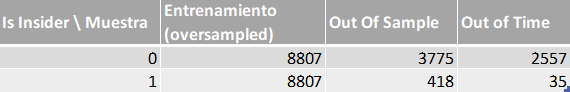
\includegraphics[width=0.5\textwidth]{imagenes/Muestras.PNG}
    \caption{Observaciones por muestra}
    \label{fig:muestras}
\end{figure}


Para cada modelo, se utilizó una reducción de dimensión conocida como Eliminación Recursiva de Atributos, el cual es un proceso iterativo que ordena las variables a partir de la importancia en el modelo a partir de una métrica. Más aún, para cada modelo, se utilizó un método de validación cruzada y selección de hiperparámetros con métodos de búsqueda en red y aleatorio, utilizando la validación cruzada como medio para evitar el sobreajuste, y afinar los métodos para escoger la mejor configuración o arquitectura.

Una vez que se tuvo listo cada modelo, después de entrenado, se aplicó la predicción sobre las muestras ``Out of Sample'' y ``Out of time'', verificando la matriz de confusión para seleccionar los mejores modelos a partir de la precisión del modelo pero el ajuste fino, en este caso, será el ``recall'', ya que por la naturaleza de los datos y su desbalance, será una mejor métrica de selección, ya que los casos son muy escasos a pesar de la gran cantidad de información, lo que debería de afinar el ``recall''. Se muestra la matriz de confusión esta métrica.

\begin{figure}[h]
    \centering
    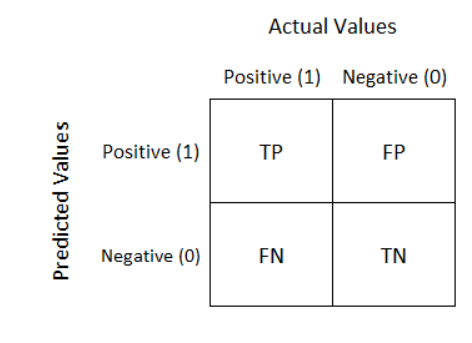
\includegraphics[width=0.6\textwidth]{imagenes/confusionMatrix.PNG}
    \caption{Matriz de Confusión}
    \label{fig:confusionMatrix}
\end{figure}

De aquí, que nuestro ``recall'' estará dado por $\frac{TP}{TP+FN}$ , esto nos dice de todas las clases positivas, ¿Cuántos predijo correctamente?, de esta forma, mejorar la selección aleatoria de sujetos y reducir el riesgo de tener un ``insider'' y no clasificarlo debidamente.

\section{Resultados y discusión}
\label{sec:resultados}

Se pueden observar variables muy correlacionadas a partir de las etiquetas observadas, podemos observar en la figura \ref{fig:pairPlot} algunas de las variables más importantes, que se reflejan en relación con la etiqueta ``isInsider'', la cual nos marca las observaciones que han sido detectadas como ``insiders''.

\begin{figure}[h]
    \centering
    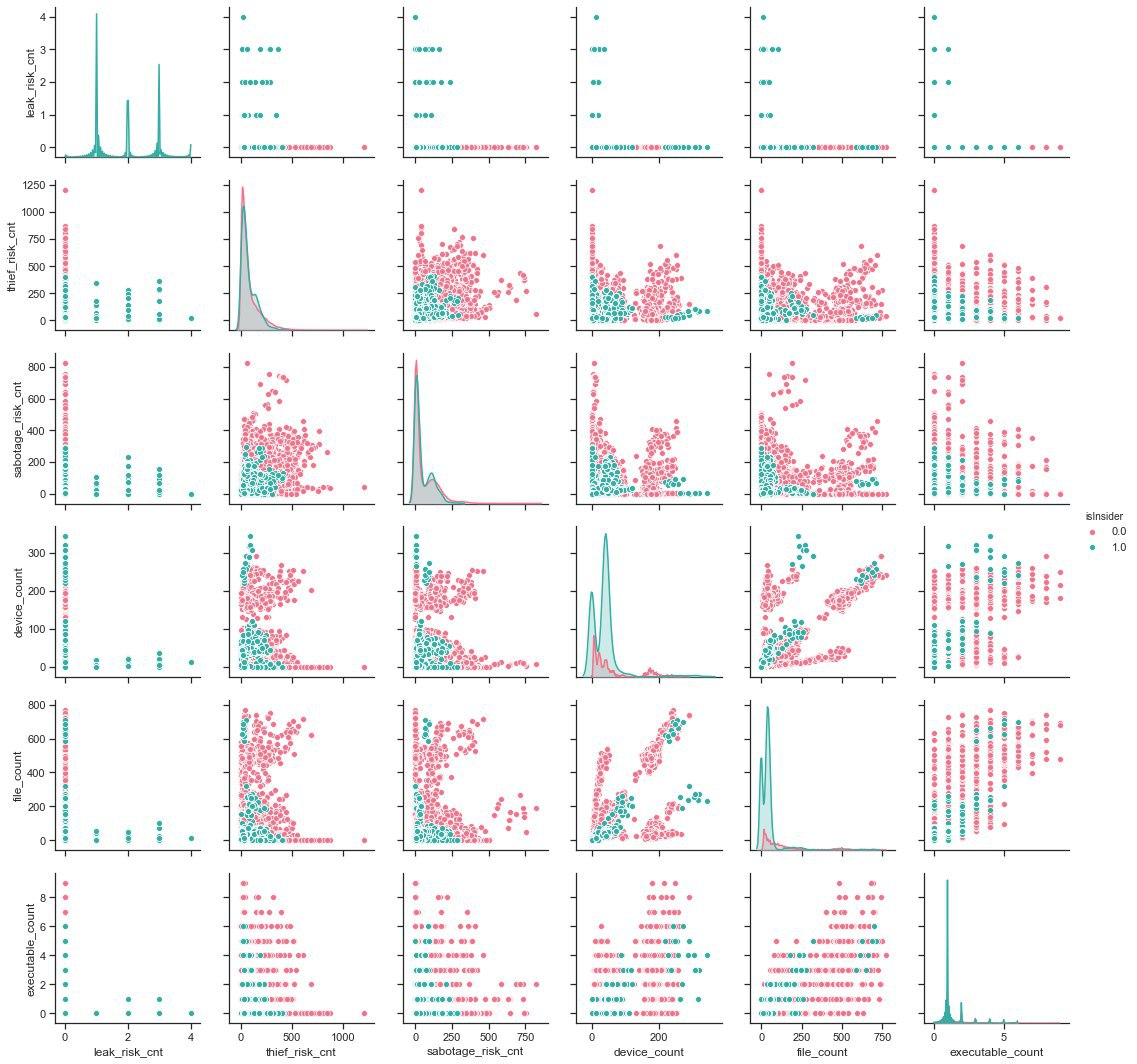
\includegraphics[width=1\textwidth]{imagenes/PairPlot.PNG}
    \caption{Relación entre variables y etiqueta}
    \label{fig:pairPlot}
\end{figure}

Si se hace una observación más detenida, podemos ver que los ``insiders'', mayormente hacen sus transacciones en horario laboral (8 AM a 5 PM), pero, observando a la gente que se queda a trabajar fuera de horario, los perpetradores son mayoría (Figura \ref{fig:inisiderHours}) aunque la muestra es mucho menor. También se puede observar que ningún perpetrador es supervisor (Figura \ref{fig:supervisors}) y los temas de sitios que visitan son muy específicos (Figura \ref{fig:insidersites}).

\begin{figure}
    \centering
    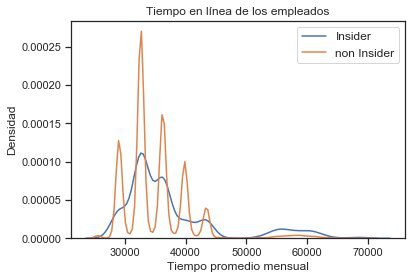
\includegraphics[width = 1\textwidth]{imagenes/InsiderHours.PNG}
    \caption{Conteo de perpetradores y horas de trabajo.}
    \label{fig:inisiderHours}
\end{figure}

\begin{figure}
    \centering
    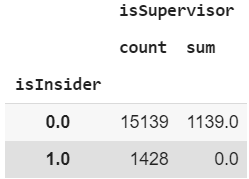
\includegraphics[width = 0.4\textwidth]{imagenes/isSupervisor.PNG}
    \caption{Conteo de supervisores.}
    \label{fig:supervisors}
\end{figure}

\begin{figure}
    \centering
    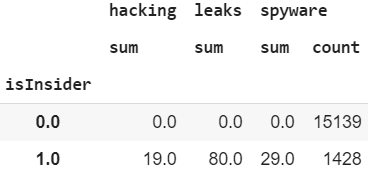
\includegraphics[width = 0.6\textwidth]{imagenes/InsiderSites.PNG}
    \caption{Sitios que visitan los perpetradores.}
    \label{fig:insidersites}
\end{figure}

Se presentan los resultados de la comparación de los modelos, y se muestra que el método de Random Forest parece ser mejor para detectar perpetradores con la mejor precisión en ambas muestras (OoS [Figura \ref{fig:oos}]  y OoT [Figura \ref{fig:oot}]), mientras que SVM pareciese tener un buen desempeño (Figura \ref{fig:svmOos}), es engañoso, ya que al ver a detalle el reporte y la matriz de confusión, podemos ver que en la muestra OoT (Figura \ref{fig:svmOot}) no funciona, y por tanto quedará descartado en el análisis. 

\begin{figure}
    \centering
    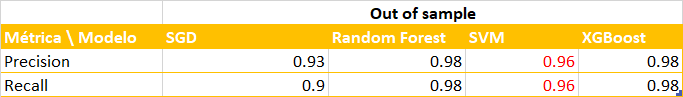
\includegraphics[width = 0.7\textwidth]{imagenes/Out_of_Sample.png}
    \caption{Out of Sample}
    \label{fig:oos}
\end{figure}

\begin{figure}
    \centering
    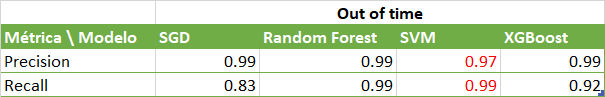
\includegraphics[width = 0.7\textwidth]{imagenes/Out_of_time.png}
    \caption{Out of Time}
    \label{fig:oot}
\end{figure}

\begin{figure}
    \centering
    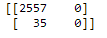
\includegraphics[width = 0.4\textwidth]{imagenes/CM_OOT_SMV.PNG}
    \caption{Matriz de confusión OoT de SVM}
    \label{fig:svmcm}
\end{figure}

\begin{figure}
    \centering
    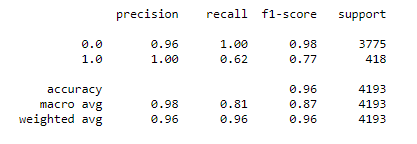
\includegraphics[width = 0.7\textwidth]{imagenes/SVM_OSS.PNG}
    \caption{Reporte de clasificación SVM OoS}
    \label{fig:svmOos}
\end{figure}

\begin{figure}
    \centering
    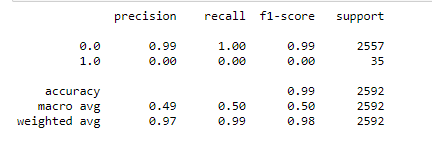
\includegraphics[width = 0.7\textwidth]{imagenes/SVM_OOT.PNG}
    \caption{Reporte de clasificación SVM OoT}
    \label{fig:svmOot}
\end{figure}

Es de importancia, en la selección de las muestras para analizar el modelo, utilizar una muestra fuera de tiempo, ya que ha sido un factor para descartar el modelo por su bajo desempeño. 

\section{Conclusiones}
\label{sec:conclusions}

Para este conjunto de datos, pareciese ser que los mejores modelos se basan en árboles de decisión, teniendo un desempeño superior a las SVM y al SGD, compartiendo parte de este resultado con \cite{noever2019classifier}. Se propone extender este trabajo reduciendo la granularidad de los datos y tal vez con datos exógenos, como factores sociodemográficos de los usuarios, situación en burós de crédito y actualizar con cierta periodicidad los artefactos psicométricos de caracterización de la personalidad. 

Se puede ver que el comportamiento de los ``insiders'' parece reflejarse en su huella digital y en su comportamiento en las oficinas, siendo que visitan sitios específicos y algunos se quedan a utilizar el equipo de trabajo después de la hora regular de salida, mientras que ninguno ha tenido un puesto importante dentro del organigrama de la empresa.

Desde el punto de vista de aprendizaje máquina, se podría intentar aprendizaje por refuerzo y aprendizaje profundo, que está fuera del contexto de este proyecto. Aprendizaje profundo nos podría dar la ventaja de detectar a los perpetradores con una granularidad de datos más pequeña, pues se podrían utilizar como observaciones datos no agrupados como se hizo en este proyecto, y generar más varianza en la información, ya que entendido el subtexto de la agrupación mensual, se tendría que calificar las observaciones con una regularidad de un mes mientras que en el otro caso se podrían calificar en tiempo real. 

Finalmente, basado en la experiencia profesional de los autores, estos consideran que el crimen financiero debe de ser analizado desde diferentes perspectivas y un único modelo no mitiga el riesgo totalmente, un programa de prevención de dicho riesgo debe contener modelos supervisados para la detección de tipologías, como las presentadas en este trabajo; modelos no supervisados, para la detección de nuevas tipologías; un modelo del comportamiento de clientes y empleados a través de tiempo, y uno que modele las relaciones de clientes o empleados con otros agentes.

\bibliographystyle{splncs04}
\bibliography{bibliografia/article}

\end{document}
